\documentclass[tikz,border=8pt]{standalone}
\usetikzlibrary{arrows.meta,positioning}
\definecolor{blue}{HTML}{0072B2}\definecolor{orange}{HTML}{E69F00}
\definecolor{green}{HTML}{009E73}\definecolor{red}{HTML}{D55E00}
\definecolor{purple}{HTML}{CC79A7}\definecolor{ink}{HTML}{172033}
\begin{document}
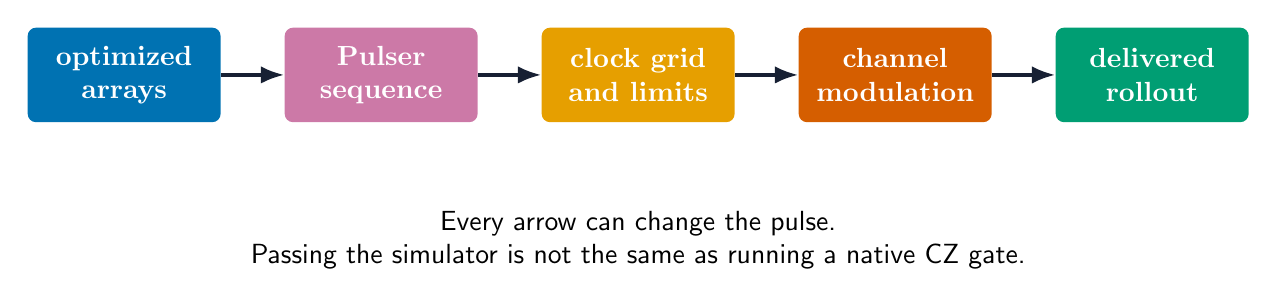
\begin{tikzpicture}[font=\sffamily,>=Latex,node distance=8mm,
box/.style={rounded corners=3pt,minimum width=2.45cm,minimum height=1.2cm,align=center,text=white,font=\bfseries}]
 \node[box,fill=blue] (array) {optimized\\arrays};
 \node[box,fill=purple,right=of array] (pulse) {Pulser\\sequence};
 \node[box,fill=orange,right=of pulse] (clock) {clock grid\\and limits};
 \node[box,fill=red,right=of clock] (filter) {channel\\modulation};
 \node[box,fill=green,right=of filter] (rollout) {delivered\\rollout};
 \draw[->,very thick,ink] (array) -- (pulse);
 \draw[->,very thick,ink] (pulse) -- (clock);
 \draw[->,very thick,ink] (clock) -- (filter);
 \draw[->,very thick,ink] (filter) -- (rollout);
 \node[below=1cm of clock,align=center] {Every arrow can change the pulse.\\Passing the simulator is not the same as running a native CZ gate.};
\end{tikzpicture}
\end{document}
